% !TeX program = xelatex
\documentclass[10pt]{beamer}

\usetheme{metropolis}

\usepackage{pgfplots}
\usepgfplotslibrary{fillbetween}
\usepackage{pgfopts}
\usepackage{amsmath}
\usepackage{structuralanalysis}
\usepackage{tikz}
\usepackage{tikz-3dplot}
\usepackage{chngcntr}
\usepackage{wasysym}
\usepackage{mathtools}
\usepackage{alphalph}
\usepackage{xcolor}
\usepackage[showdow=false, en-US]{datetime2}
\usepackage{hyperref}

\newcommand{\highlight}[1]{%
	\colorbox{red!50}{$\displaystyle#1$}}

\setcounter{lecture}{13}
\counterwithin{equation}{lecture}
\makeatletter
\def\user@resume{resume}
\def\user@intermezzo{intermezzo}
%
\newcounter{previousequation}
\newcounter{lastsubequation}
\newcounter{savedparentequation}
\setcounter{savedparentequation}{1}
% 
\renewenvironment{subequations}[1][]{%
	\def\user@decides{#1}%
	\setcounter{previousequation}{\value{equation}}%
	\ifx\user@decides\user@resume 
	\setcounter{equation}{\value{savedparentequation}}%
	\else  
	\ifx\user@decides\user@intermezzo
	\refstepcounter{equation}%
	\else
	\setcounter{lastsubequation}{0}%
	\refstepcounter{equation}%
	\fi\fi
	\protected@edef\theHparentequation{%
		\@ifundefined {theHequation}\theequation \theHequation}%
	\protected@edef\theparentequation{\theequation}%
	\setcounter{parentequation}{\value{equation}}%
	\ifx\user@decides\user@resume 
	\setcounter{equation}{\value{lastsubequation}}%
	\else
	\setcounter{equation}{0}%
	\fi
	\def\theequation  {\theparentequation  \alph{equation}}%
	\def\theHequation {\theHparentequation \alph{equation}}%
	\ignorespaces
}{%
%  \arabic{equation};\arabic{savedparentequation};\arabic{lastsubequation}
\ifx\user@decides\user@resume
\setcounter{lastsubequation}{\value{equation}}%
\setcounter{equation}{\value{previousequation}}%
\else
\ifx\user@decides\user@intermezzo
\setcounter{equation}{\value{parentequation}}%
\else
\setcounter{lastsubequation}{\value{equation}}%
\setcounter{savedparentequation}{\value{parentequation}}%
\setcounter{equation}{\value{parentequation}}%
\fi\fi
%  \arabic{equation};\arabic{savedparentequation};\arabic{lastsubequation}
\ignorespacesafterend
}
\makeatother
\title{AE 737 - Mechanics of Damage Tolerance}
\subtitle{Lecture \arabic{lecture}}
\date{Last Updated: \today\ at \DTMcurrenttime}
\author{Dr. Nicholas Smith}
\institute{Wichita State University, Department of Aerospace Engineering}
% \titlegraphic{\hfill\includegraphics[height=1.5cm]{logo/logo}}

\begin{document}

\maketitle
\begin{frame}{schedule}
	\begin{itemize}
		\item 3 Mar - Section 1 Review, Homework 5 return
		\item 8 Mar - Exam 1
		\item 10 Mar - Exam return, Final Project discussion
		\item 22 Mar - Stress based fatigue, Homework 6 assigned
		\item 24 Mar - Stress based fatigue
	\end{itemize}
\end{frame}

\begin{frame}
  \frametitle{outline}
  \setbeamertemplate{section in toc}[sections numbered]
  \tableofcontents[hideallsubsections]
\end{frame}

\section{exam notes}

\begin{frame}{exam}
	\begin{itemize}[<+->]
		\item 4 questions
		\item Bring a scientific calculator (or graphing)
		\item Specific equations or correction factors (i.e. modified MSD or $\beta$ for stiffeners) will be given where needed
		\item Equation sheet is posted on Blackboard
	\end{itemize}
\end{frame}

\section{stress intensity}

\begin{frame}{methods for finding stress intensity}
	\begin{itemize}[<+->]
		\item Handbook lookup
		\item Superposition
		\item Compounding
		\item Stress concentration ratio
		\item Stress function method (Westergaard)
		\item Boundary collocation (approximation to Westergaard)
		\item Schwartz-Neumann alternating method (approximation to Westergaard)
		\item Finite elements (Direct, Modified Crack Closure)
		\item Boundary elements
		\item Experimental
	\end{itemize}
\end{frame}

\begin{frame}{superposition}
	\begin{itemize}
		\item Since the stress intensity factor is derived using Linear Elasticity, the principle of superposition applies
		\item Multiple applied loads can be superposed to find the effective stress intensity factor of the combined loading
	\end{itemize}
\end{frame}

\begin{frame}{superposition}
	\begin{figure}[H]
		\begin{tikzpicture}
		\point{a}{0}{1.5};
		\point{b}{3}{1.5};
		\point{c}{0}{-2};
		\point{d}{3}{-2};
		\draw (0,0) -- (0,1) -- (3,1) -- (3,-1) -- (0,-1) -- (0,0);
		\draw (1,0) -- (2,0);
		\draw node at (1.5,0.2) {2a};
		\lineload{3}{a}{b}[-.5][-.5];
		\draw node at (1.5,2) {$\sigma$};
		\lineload{3}{c}{d}[.5][.5];
		\draw node at (1.5,-2) {$\sigma$};
		\draw [->] (1.5,.5) -- (1.5,0.8) node[right] {$P$};
		\draw [->] (1.5,-.5) -- (1.5,-0.8) node[right] {$P$};
		\draw[fill=black] (1.5,.5) circle (0.03);
		\draw[fill=black] (1.5,-.5) circle (0.03);
		\draw[<->] (0.5,0) -- (0.5,0.5);
		\draw[<->] (0.5,0) -- (0.5,-0.5);
		\draw node at (0.3,0.25) {S} node at (0.3,-0.25) {S};
		\draw node at (3.5,0) {=};
		\point{e}{4}{1.5};
		\point{f}{7}{1.5};
		\point{g}{4}{-2};
		\point{h}{7}{-2};
		\draw (4,0) -- (4,1) -- (7,1) -- (7,-1) -- (4,-1) -- (4,0);
		\draw (5,0) -- (6,0);
		\draw node at (5.5,0.2) {2a};
		\lineload{3}{e}{f}[-.5][-.5];
		\draw node at (5.5,2) {$\sigma$};
		\lineload{3}{g}{h}[.5][.5];
		\draw node at (5.5,-2) {$\sigma$};
		\draw node at (7.5,0) {+};
		\draw (8,0) -- (8,1) -- (11,1) -- (11,-1) -- (8,-1) -- (8,0);
		\draw (9,0) -- (10,0);
		\draw node at (9.5,0.2) {2a};
		\draw [->] (9.5,.5) -- (9.5,0.8) node[right] {$P$};
		\draw [->] (9.5,-.5) -- (9.5,-0.8) node[right] {$P$};
		\draw[fill=black] (9.5,.5) circle (0.03);
		\draw[fill=black] (9.5,-.5) circle (0.03);
		\draw[<->] (8.5,0) -- (8.5,0.5);
		\draw[<->] (8.5,0) -- (8.5,-0.5);
		\draw node at (8.3,0.25) {S} node at (8.3,-0.25) {S};
		\end{tikzpicture}
	\end{figure}
\end{frame}

\begin{frame}{superposition}
	\begin{align*}
	K_I &= K_{I(\sigma)} + K_{I(P)}\\
	K_I &= \sigma\sqrt{\pi a} + \frac{P}{t\sqrt{\pi a}}\frac{1 - 0.5\left(\frac{a}{W}\right)+0.975\left(\frac{a}{W}\right)^2 - 0.16\left(\frac{a}{W}\right)^3}{\sqrt{1-\left(\frac{a}{W}\right)}}
	\end{align*}
\end{frame}

\begin{frame}{superposition}
	\begin{itemize}
		\item Sometimes, the superposition needed to solve a problem is not obvious
		\item It can be helpful to subtract a known solution from the problem
	\end{itemize}
\end{frame}

\begin{frame}{superposition}
	\begin{figure}[H]
		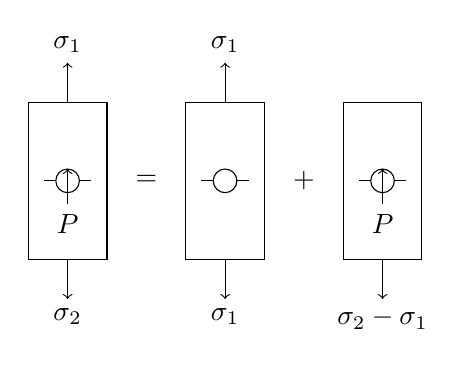
\begin{tikzpicture}
		\draw (0,-1) -- (0,1) -- (1,1) -- (1,-1) -- (0,-1);
		\draw[->] (0.5,1) -- (0.5,1.5) node[above] {$\sigma_1$};
		\draw[->] (0.5,-1) -- (0.5,-1.5) node[below] {$\sigma_2$};
		\draw (0.5,0) circle (0.15);
		\draw (0.35,0) -- (0.2,0);
		\draw (0.65,0) -- (0.8,0);
		\draw[->] (0.5,-0.3) node[below] {$P$} -- (0.5,0.15);
		\draw node at (1.5,0) {=};
		\draw (2,-1) -- (2,1) -- (3,1) -- (3,-1) -- (2,-1);
		\draw[->] (2.5,1) -- (2.5,1.5) node[above] {$\sigma_1$};
		\draw[->] (2.5,-1) -- (2.5,-1.5) node[below] {$\sigma_1$};
		\draw (2.5,0) circle (0.15);
		\draw (2.35,0) -- (2.2,0);
		\draw (2.65,0) -- (2.8,0);
		\draw node at (3.5,0) {+};
		\draw (4,-1) -- (4,1) -- (5,1) -- (5,-1) -- (4,-1);
		\draw[->] (4.5,-1) -- (4.5,-1.5) node[below] {$\sigma_2-\sigma_1$};
		\draw (4.5,0) circle (0.15);
		\draw (4.35,0) -- (4.2,0);
		\draw (4.65,0) -- (4.8,0);
		\draw[->] (4.5,-0.3) node[below] {$P$} -- (4.5,0.15);
		\end{tikzpicture}
	\end{figure}
\end{frame}

\begin{frame}{superposition}
	\begin{figure}[H]
		\centering
		\begin{tikzpicture}
		\begin{scope}[scale=2, shift={(-2,0)}]
		\point{a}{6}{-3.25};
		\point{b}{8}{-3.25};
		\draw (3,-1) -- (3,1) -- (4,1) -- (4,-1) -- (3,-1);
		\draw (3.3,0) -- (3.7,0);
		\draw[->] (3.5,0.2) -- (3.5,0.6) node[above] {P};
		\draw node at (3.5,-0.1) {$2a$};
		\lineload{3}{a}{b}[.25][.25];
		\draw node at (3.5,-1.5) {$\sigma$};
		\end{scope}
		\end{tikzpicture}
	\end{figure}
\end{frame}

\section{fracture toughness}

\begin{frame}{fracture toughness}
	\begin{itemize}
		\item The critical load at which a cracked specimen fails produces a critical stress intensity factor
		\item The "critical stress intensity factor" is known as $K_c$
		\item For Mode I, this is called $K_{Ic}$
		\item The critical stress intensity factor is also known as fracture toughness
		\begin{equation}
		K_{IC} = \sigma_c \sqrt{\pi a}\beta
		\end{equation}
		\pause
		\item NOTE: "Fracture Toughness" can also refer to $G_{Ic}$, which is analogous to $K_{Ic}$, but not the same
	\end{itemize}
\end{frame}

\begin{frame}{fracture toughness}
	\begin{itemize}
		\item Fracture toughness is a material property, but it is only well-defined in certain conditions
		\item Brittle materials
		\item Plane strain (smaller plastic zone)
		\item In these cases ASTM E399-12 is used.
	\end{itemize}
\end{frame}

\begin{frame}{fracture toughness}
	\begin{figure}
		\centering
		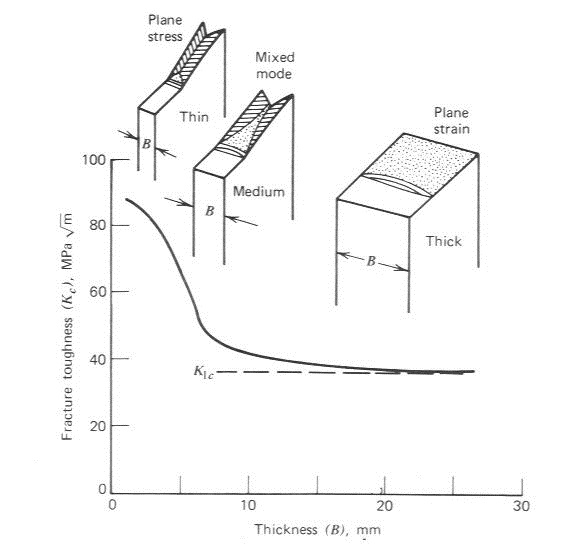
\includegraphics[width=0.7\linewidth]{KIC_thickness}
		\label{fig:KIC_thickness}
	\end{figure}
\end{frame}

\begin{frame}{fracture toughness}
	\begin{itemize}[<+->]
		\item "Stable" vs. "unstable" crack growth
		\item Stable crack growth means the crack extends only with increased load
		\item Unstable crack growth means the crack will continue to extend indefinitely under the same load
		\item For a perfectly brittle material, there is no stable crack growth, as soon as a critical load is reached, the crack will extend indefinitely
		\item For an elastic-plastic material, once the load is large enough to extend the crack, it will extend slightly
		\item The load must be continually increased until a critical value causes unstable crack growth
	\end{itemize}
\end{frame}

\begin{frame}{fracture toughness}
	\begin{itemize}[<+->]
		\item During an experiment, we will record the crack length and applied load ($P_i$, $a_i$) each time we increase the load
		\item We can calculate a unique stress intensity factor $K_{Ii}$ at each of these points
		\item These are then used to create a "K-curve", plotting $K_I$ vs. $a$
	\end{itemize}
\end{frame}

\begin{frame}{K-curve}
	\begin{figure}
		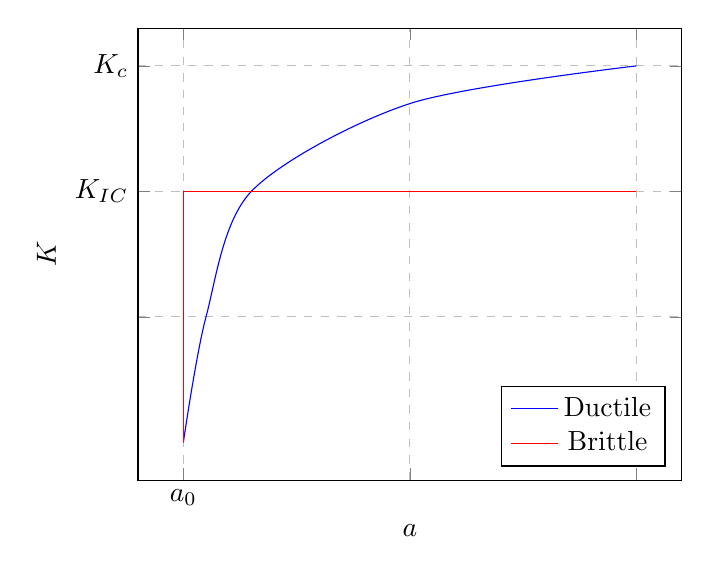
\begin{tikzpicture}
		\begin{axis}[
		width=0.7\linewidth,
		grid=major,
		grid style=dashed,
		xlabel=$a$,
		ylabel=$K$,
		xtick={1,2,3},
		xticklabels={$a_0$, , },
		ytick={0.5,1,1.5},
		yticklabels={ ,$K_{IC}$,$K_c$},
		legend entries={Ductile, Brittle},
		legend pos=south east,
		no markers
		]
		\addplot+[smooth]
		coordinates
		{(1,0) (1.1,0.5) (1.3,1) (2,1.35) (3,1.5)};
		\addplot+[const plot]
		coordinates
		{(1,0) (1,1) (3,1)};
		\end{axis}
		\end{tikzpicture}
	\end{figure}
\end{frame}

\begin{frame}{$K_R$ Curve}
	
\begin{figure}
\centering
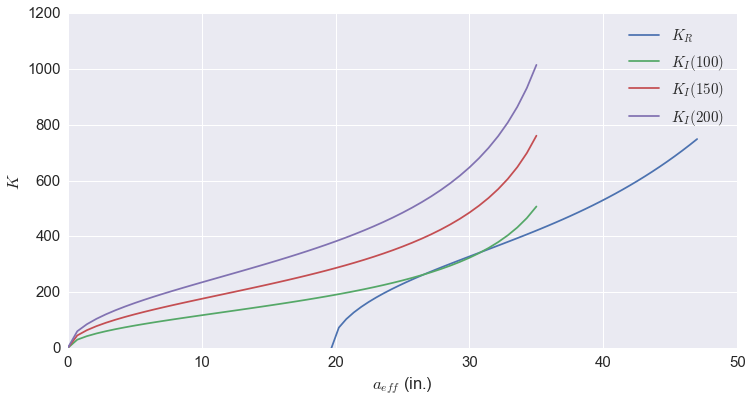
\includegraphics[width=0.8\linewidth]{KR_curve}
\label{fig:KR_curve}
\end{figure}
\end{frame}

\section{residual strength}

\begin{frame}{residual strength}
	\begin{itemize}[<+->]
		\item In the last chapter we performed some basic residual strength analysis by checking for net section yield
		\item As the crack grows, the area of the sample decreases, increasing the net section stress
		\item The residual strength, $\sigma_R$ is given in terms of the gross area, so as the crack grows the residual strength due to yield decreases
		\item We can relate the net-section stress to $\sigma_R$ by
		\begin{equation}
		\sigma_R = \sigma_{YS} \frac{A_{net}}{A_{gross}}
		\end{equation}
	\end{itemize}
\end{frame}

\begin{frame}{residual strength}
	\begin{figure}
		\begin{tikzpicture}
		\begin{axis}[domain=0:1,
		xlabel=$a/W$,
		ylabel=Residual Strength $\sigma_R$,
		ytick={0, 2},
		yticklabels={0, $\sigma_{YS}$ }]
		\addplot[mark=none,style=dashed] {-2*x + 2};
		\end{axis}
		\end{tikzpicture}
	\end{figure}
\end{frame}

\begin{frame}{residual strength}
	\begin{itemize}[<+->]
		\item For brittle fracture to occur, we need to satisfy the condition
		\item
		\begin{equation}
		\sigma_R = \sigma_C = \frac{K_C}{\sqrt{\pi a}\beta}
		\end{equation}
	\end{itemize}
\end{frame}

\begin{frame}{residual strength}
	\begin{figure}
		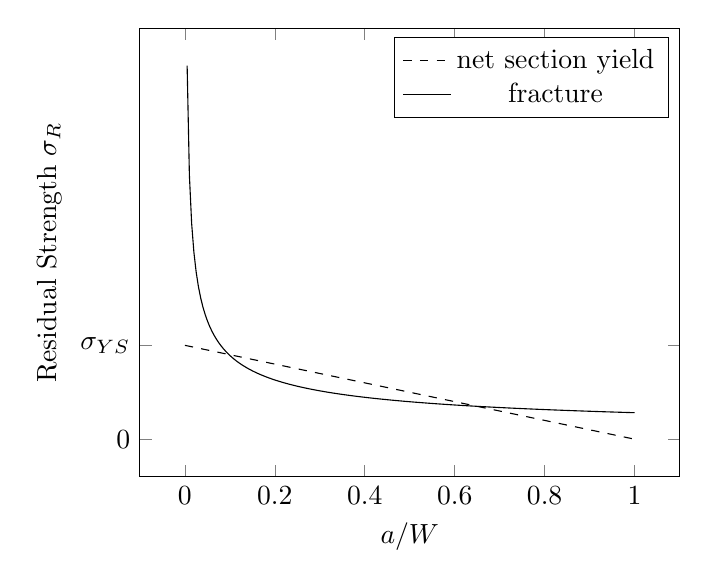
\begin{tikzpicture}
		\begin{axis}[domain=0:1,
		samples=200,
		xlabel=$a/W$,
		ylabel=Residual Strength $\sigma_R$,
		ytick={0, 2},
		yticklabels={0, $\sigma_{YS}$ }]
		\addplot[mark=none,style=dashed] {-2*x + 2};
		\addlegendentry{net section yield}
		\addplot[mark=none] {1/sqrt(3.14*x)};
		\addlegendentry{fracture}
		\end{axis}
		\end{tikzpicture}
	\end{figure}
\end{frame}

\begin{frame}{residual strength}
	\begin{itemize}[<+->]
		\item Within the same family of materials (i.e. Aluminum), there is generally a trade-off between yield stress and fracture toughness
		\item As we increase the yield strength, we decrease the fracture toughness (and vice versa)
		\item Consider a comparison of the following aluminum alloys
		\begin{enumerate}
			\item 7178-T6, $K_C = 43 \text{ ksi} \sqrt{\text{in.}}$, $\sigma_{YS} = 74 \text{ksi}$
			\item 7075-T6, $K_C = 68 \text{ ksi} \sqrt{\text{in.}}$, $\sigma_{YS} = 63 \text{ksi}$
			\item 2024-T3, $K_C = 144 \text{ ksi} \sqrt{\text{in.}}$, $\sigma_{YS} = 42 \text{ksi}$
		\end{enumerate}
	\end{itemize}
\end{frame}

\begin{frame}{residual strength}
	\begin{itemize}[<+->]
		\item As an example let us consider an edge-cracked panel with $W=6"$ and $t=0.1"$
		\item The net section yield condition will be given by
		\item 
		\begin{equation*}
		\sigma_C = \sigma_{YS} \frac{W-a}{W} = \sigma_{YS}\frac{6-a}{6}
		\end{equation*}
		\item And the fracture condition by
		\begin{equation*}
		\sigma_C = \frac{K_C}{\sqrt{\pi a} \beta}
		\end{equation*}
		With
		\begin{equation*}
		\beta = 1.12 - 0.231\left(\frac{a}{W}\right) + 10.55 \left(\frac{a}{W}\right)^2 - 21.72 \left(\frac{a}{W}\right)^3 + 30.39 \left(\frac{a}{W}\right)^4
		\end{equation*}
	\end{itemize}
\end{frame}

\begin{frame}{7178-T6}
	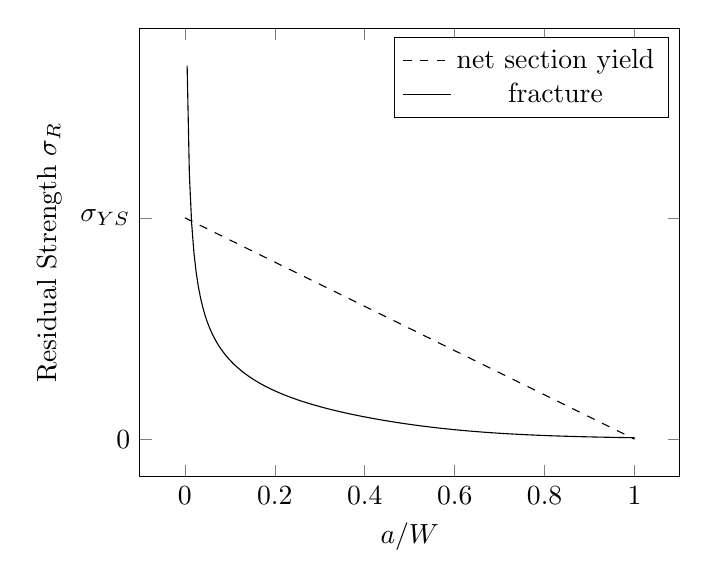
\begin{tikzpicture}
	\begin{axis}[domain=0:1,
	samples=200,
	xlabel=$a/W$,
	ylabel=Residual Strength $\sigma_R$,
	ytick={0, 74},
	yticklabels={0, $\sigma_{YS}$ }]
	\addplot[mark=none,style=dashed] {74*(1-x)};
	\addlegendentry{net section yield}
	\addplot[mark=none] {43/sqrt(3.14*x*6)/(1.12-.231*x+10.55*x^2-21.72*x^3+30.39*x^4)};
	\addlegendentry{fracture}
	\end{axis}
	\end{tikzpicture}
\end{frame}

\begin{frame}{7075-T6}
	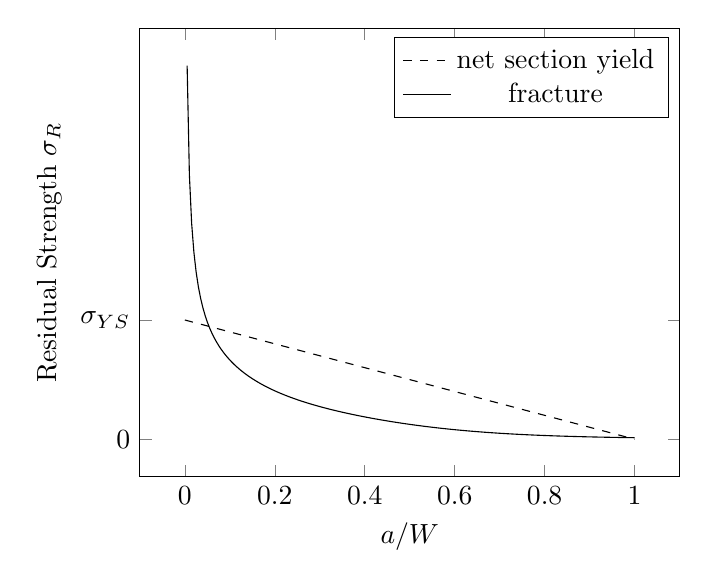
\begin{tikzpicture}
	\begin{axis}[domain=0:1,
	samples=200,
	xlabel=$a/W$,
	ylabel=Residual Strength $\sigma_R$,
	ytick={0, 63},
	yticklabels={0, $\sigma_{YS}$ }]
	\addplot[mark=none,style=dashed] {63*(1-x)};
	\addlegendentry{net section yield}
	\addplot[mark=none] {68/sqrt(3.14*x*6)/(1.12-.231*x+10.55*x^2-21.72*x^3+30.39*x^4)};
	\addlegendentry{fracture}
	\end{axis}
	\end{tikzpicture}
\end{frame}

\begin{frame}{2024-T3}
	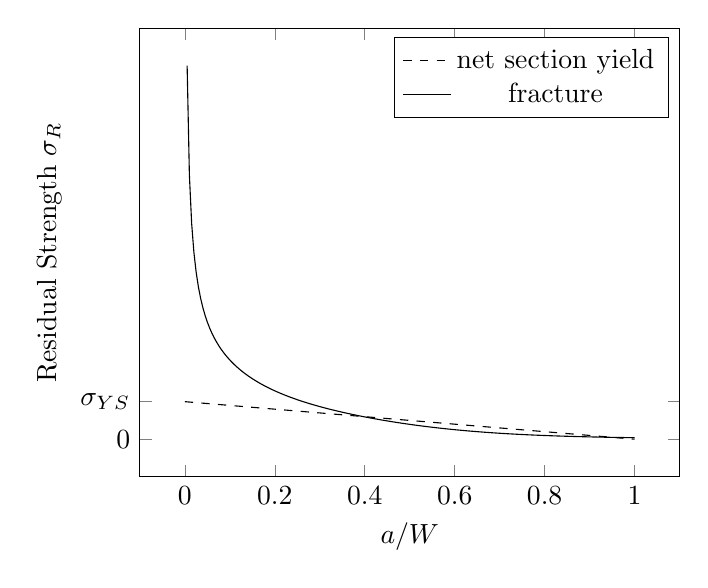
\begin{tikzpicture}
	\begin{axis}[domain=0:1,
	samples=200,
	xlabel=$a/W$,
	ylabel=Residual Strength $\sigma_R$,
	ytick={0, 42},
	yticklabels={0, $\sigma_{YS}$ }]
	\addplot[mark=none,style=dashed] {42*(1-x)};
	\addlegendentry{net section yield}
	\addplot[mark=none] {144/sqrt(3.14*x*6)/(1.12-.231*x+10.55*x^2-21.72*x^3+30.39*x^4)};
	\addlegendentry{fracture}
	\end{axis}
	\end{tikzpicture}
\end{frame}

\begin{frame}{comparison}
	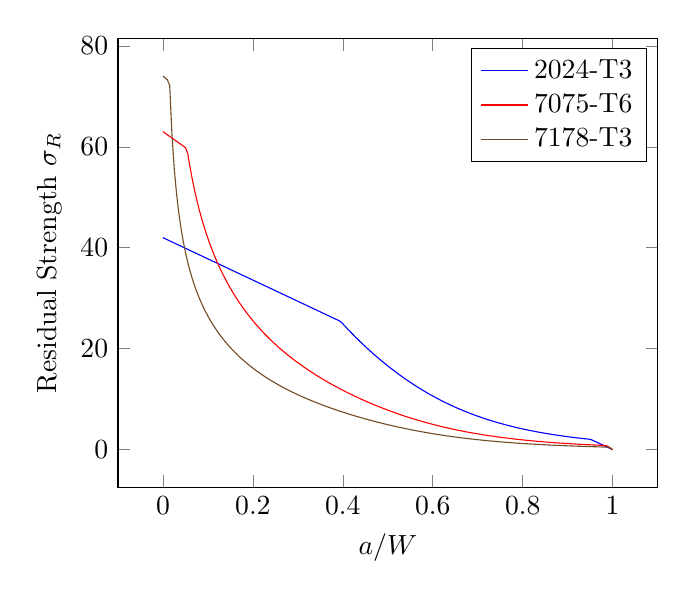
\begin{tikzpicture}
	\begin{axis}[domain=0:1,
	samples=200,
	xlabel=$a/W$,
	ylabel=Residual Strength $\sigma_R$]
	\addplot +[mark=none] {min(42*(1-x),144/sqrt(3.14*x*6)/(1.12-.231*x+10.55*x^2-21.72*x^3+30.39*x^4))};
	\addlegendentry{2024-T3}
	\addplot +[mark=none] {min(63*(1-x),68/sqrt(3.14*x*6)/(1.12-.231*x+10.55*x^2-21.72*x^3+30.39*x^4))};
	\addlegendentry{7075-T6}
	\addplot +[mark=none] {min(74*(1-x),43/sqrt(3.14*x*6)/(1.12-.231*x+10.55*x^2-21.72*x^3+30.39*x^4))};
	\addlegendentry{7178-T3}
	\end{axis}
	\end{tikzpicture}
\end{frame}

\section{stiffeners}
%stable vs. unstable crack growth
\begin{frame}{crack growth}
	\begin{itemize}[<+->]
		\item In general, residual strength curves do NOT give any information about crack growth
		\item When $\sigma_R$ is exceeded, the panel fails due to unstable crack growth
		\item Stiffeners reverse this trend to some extent, but causing some sections of residual strength curve to have positive slope
		\item When the slope of the residual strength curve is positive, crack growth is stable
		\item Thus in some cases, we can predict some amount of crack growth
	\end{itemize}
\end{frame}

\begin{frame}<handout:0>{critical crack length}
	sketch
\end{frame}

%meaning of "critical crack length"

\begin{frame}<handout:0>{residual strength}
	sketch
\end{frame}
%find panel residual strength

\section{multiple site damage}

\begin{frame}{multiple site damage}
	\begin{itemize}[<+->]
		\item Often damage can accumulate among multiple sources
		\item This is very common when there are a series of holes, each can develop cracks with a potential to link up
		\item "link up" occurs when the plastic zones between two adjacent cracks touch
	\end{itemize}
\end{frame}

%TODO redo figure
\begin{frame}{linkup}
	\begin{figure}
		\centering
		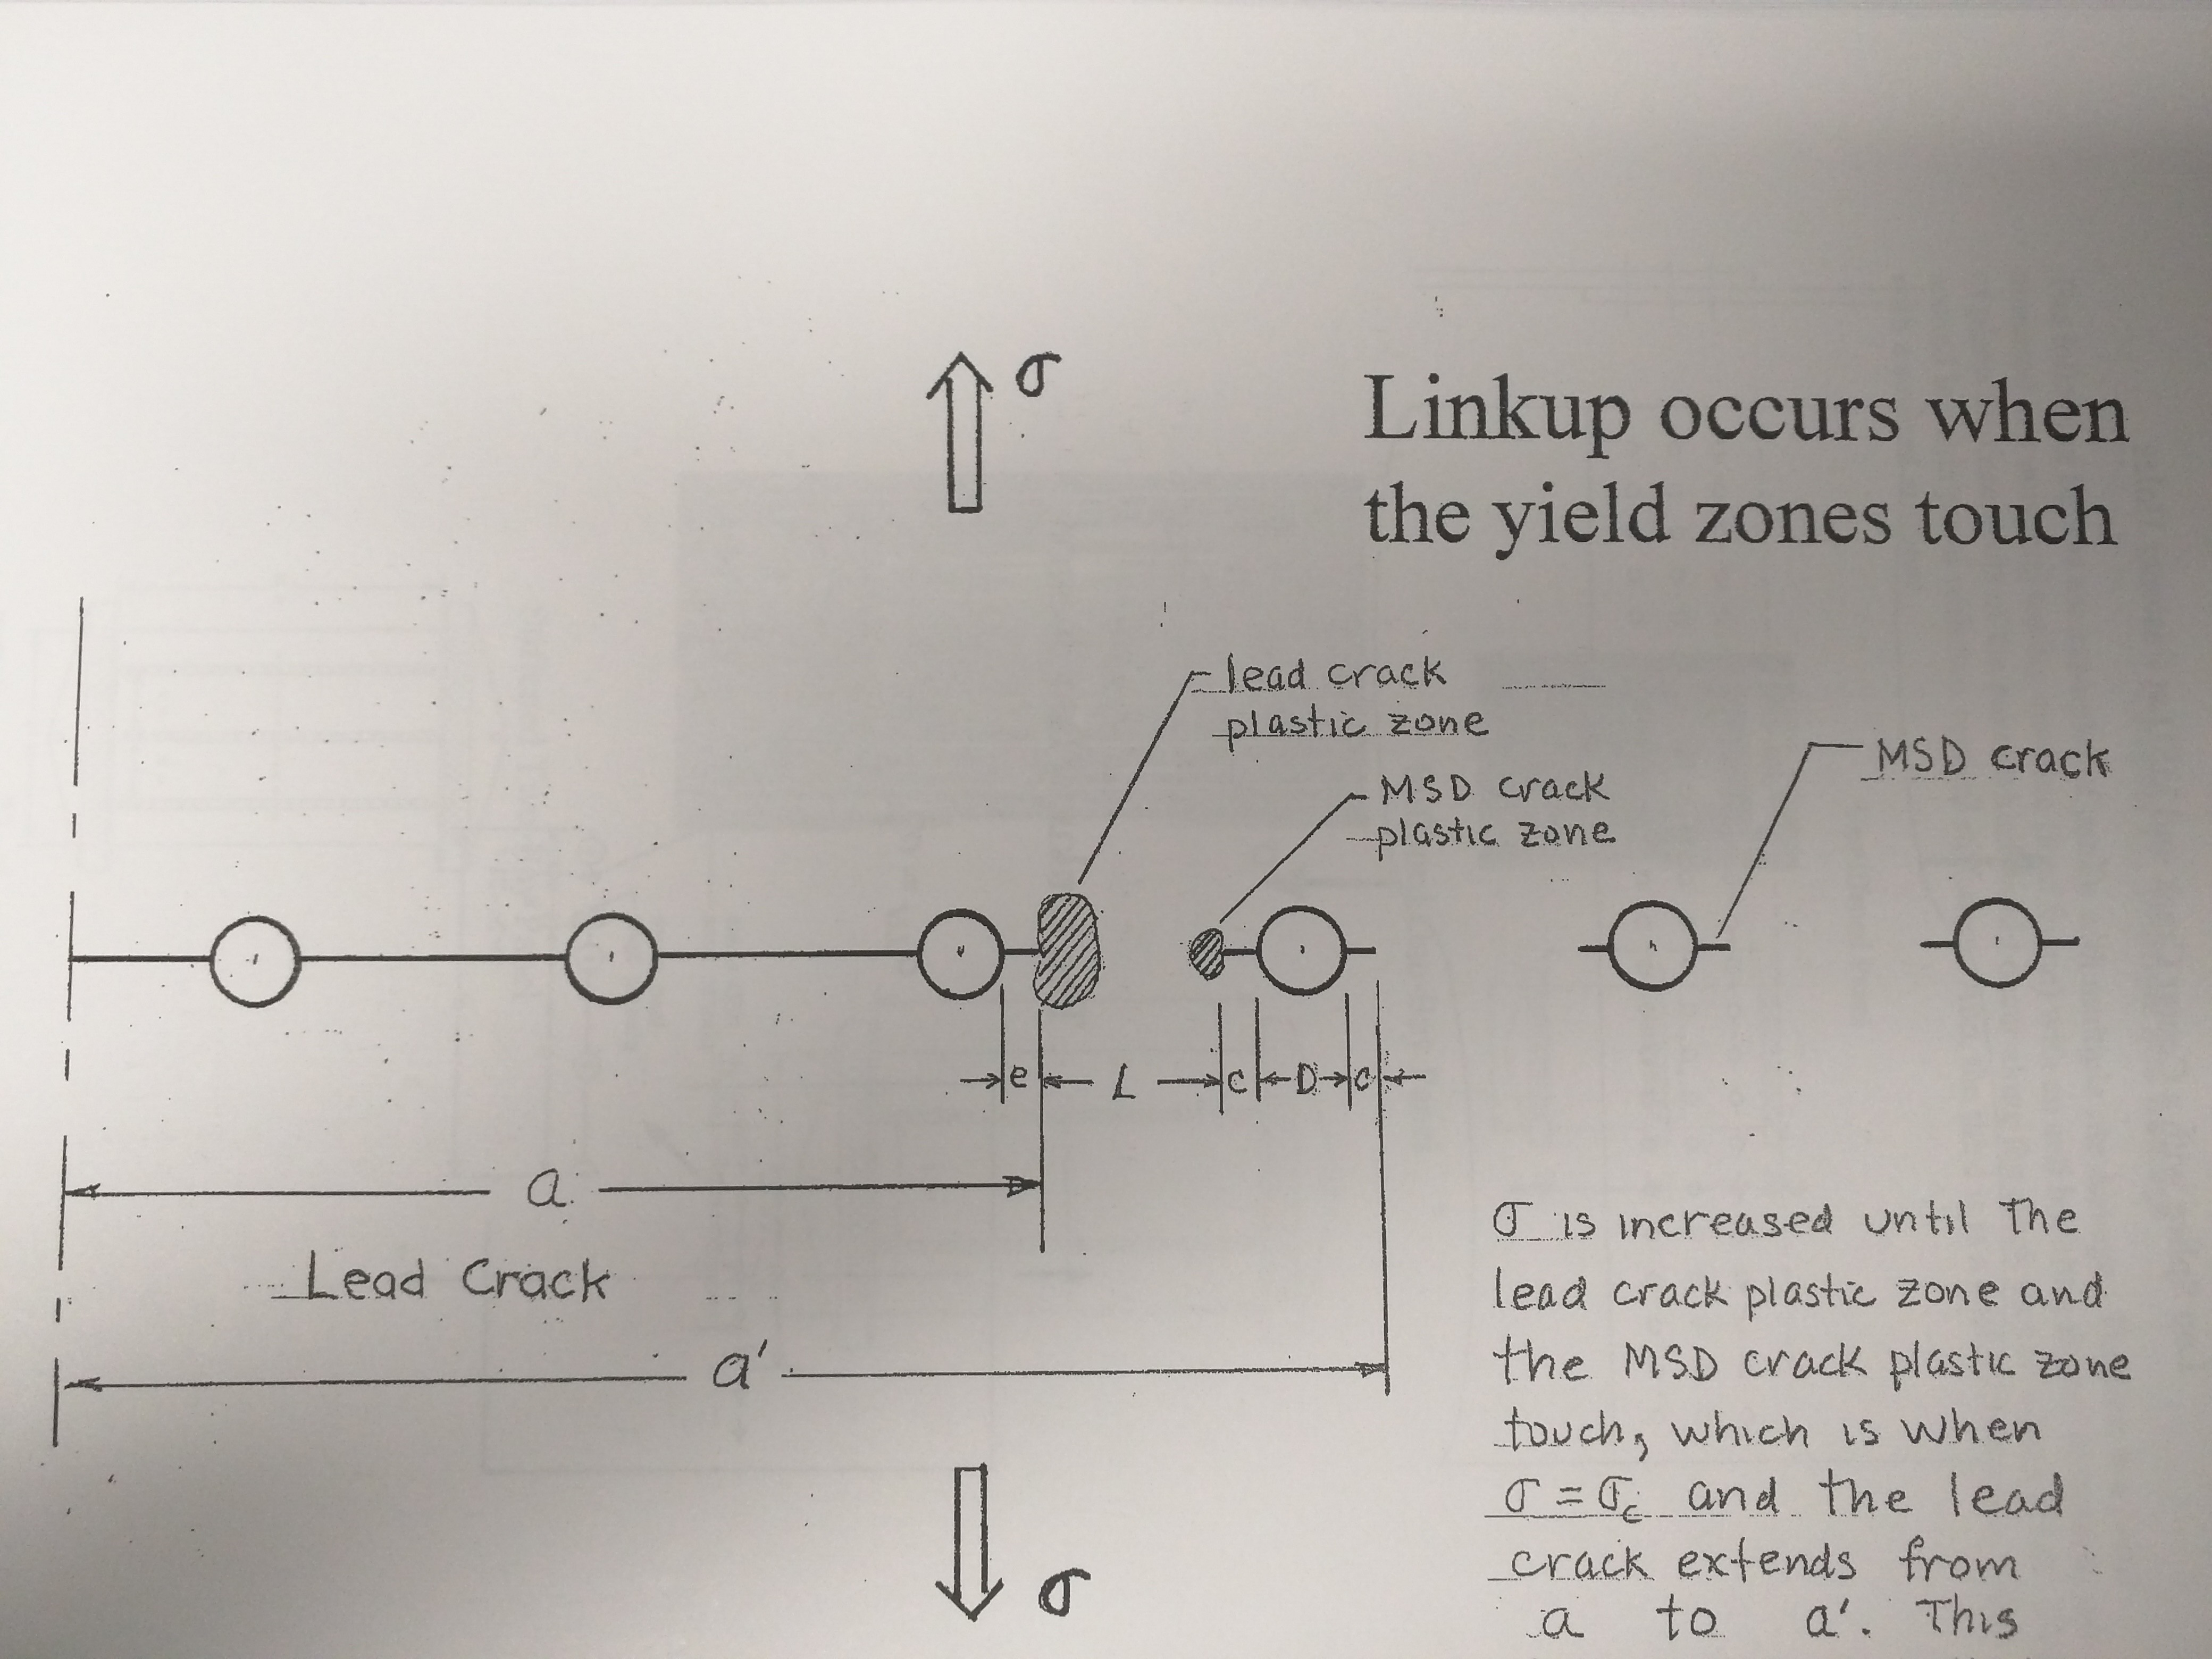
\includegraphics[width=0.7\linewidth]{msd}
		\label{fig:msd}
	\end{figure}
\end{frame}

%TODO redo figure
\begin{frame}{linkup}
	\begin{figure}
		\centering
		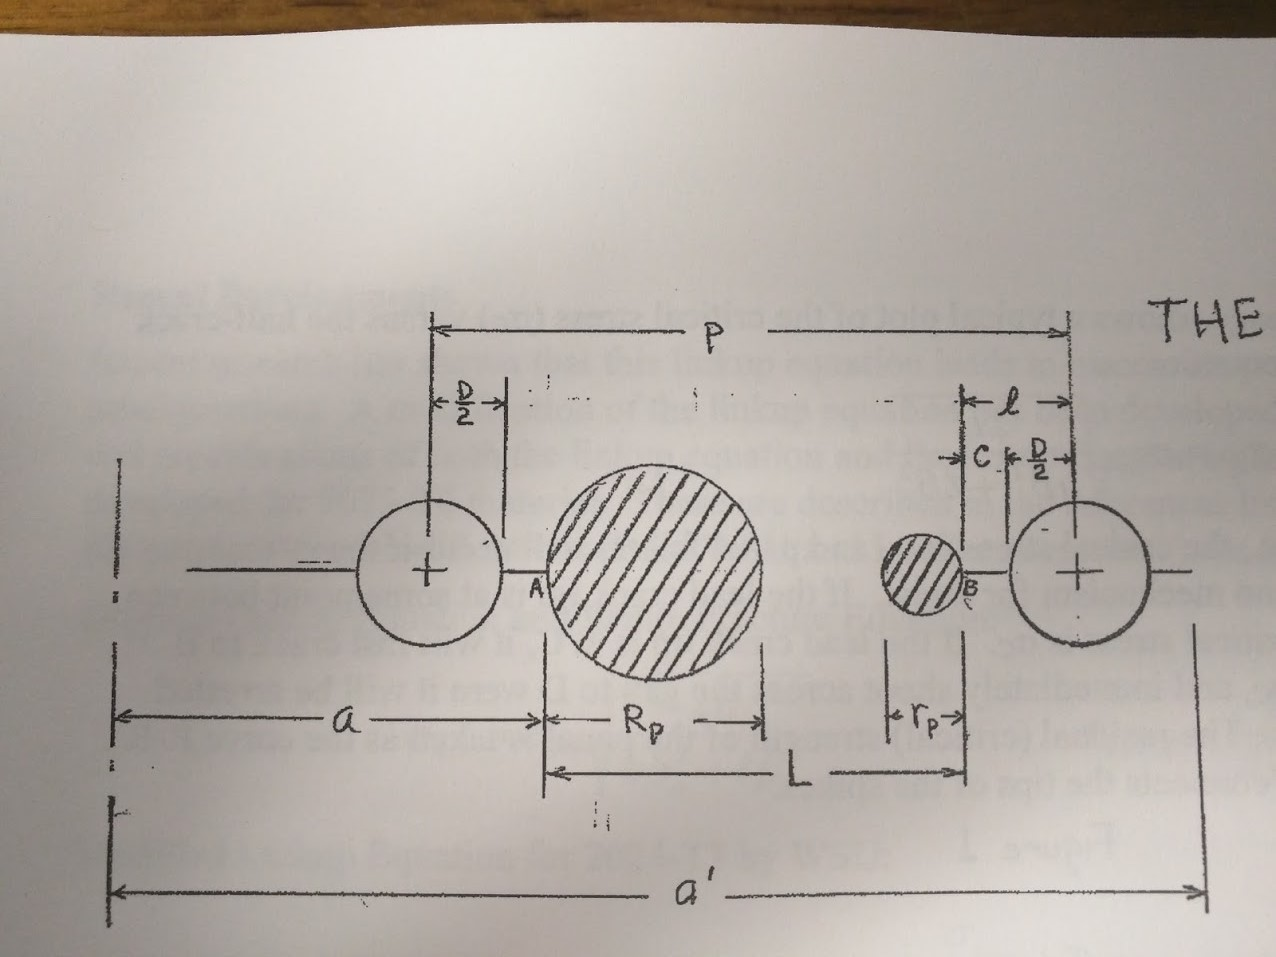
\includegraphics[width=0.7\linewidth]{linkup}
		\label{fig:linkup}
	\end{figure}
\end{frame}

\begin{frame}{linkup equation}
	\begin{itemize}[<+->]
		\item We know that
		\begin{equation}
		R_p = \frac{1}{2\pi}\left(\frac{K_{Ia}}{\sigma_{YS}}\right)^2
		\end{equation}
		\begin{equation}
		r_p = \frac{1}{2\pi}\left(\frac{K_{Il}}{\sigma_{YS}}\right)^2
		\end{equation}
		\item Where we define the stress intensity factors at a and L as
		\begin{equation}
		K_{Ia} = \sigma \sqrt{\pi a} \beta_a
		\end{equation}
		\begin{equation}
		K_{Il} = \sigma \sqrt{\pi l} \beta_l
		\end{equation}
	\end{itemize}
\end{frame}

\begin{frame}{linkup equation}
	\begin{itemize}[<+->]
		\item Since fast cracking occurs when $R_p + r_p = L$, we solve for the condition where $R_p + r_p < L$
		\begin{subequations}
			\begin{align}
			\frac{1}{2\pi}\left(\frac{K_{Ia}}{\sigma_{YS}}\right)^2 + \frac{1}{2\pi}\left(\frac{K_{Il}}{\sigma_{YS}}\right)^2 &< L\\
			\frac{1}{2\pi\sigma_{YS}^2} \left[K_{Ia}^2 + K_{Il}^2\right] &< L \\
			\frac{1}{2\pi\sigma_{YS}^2} \left[\sigma^2 \pi a \beta_a^2 + \sigma^2 \pi l \beta_l^2\right] &< L \\
			\frac{\sigma^2}{2\sigma_{YS}^2} \left[a \beta_a^2 + l \beta_l^2\right] &< L \\
			\frac{\sigma_c^2}{2\sigma_{YS}^2} \left[a \beta_a^2 + l \beta_l^2\right] &= L \\
			\label{eq:msd}
			\sigma_c &= \sigma_{YS}\sqrt{\frac{2L}{a \beta_a^2 + l \beta_l^2}}
			\end{align}
		\end{subequations}
	\end{itemize}
\end{frame}

\begin{frame}{caveats}
	\begin{itemize}
		\item The link-up equation is not a good predictor for materials with a small plastic zone size
		\item Even for ductile materials, some fine tuning of the equation is needed
		\item In practice, MSD predictions are based on experiments
	\end{itemize}
\end{frame}

\section{mixed mode fracture}

\begin{frame}{Maximum circumferential stress vs. maximum principal stress}
	\begin{itemize}[<+->]
		\item Maximum circumferential stress finds the principal stress direction near the crack tip
		\item Assumes crack will propagate due to maximum opening stress
		\item Maximum principal stress theory finds the maximum principal stress, neglecting crack tip stress field
		\item Also assumes crack propagates in Mode I direction
	\end{itemize}
\end{frame}

\section{extra credit}

\begin{frame}{digitizing figures!}
	\begin{itemize}[<+->]
		\item Our text has a lot of useful information that can be somewhat difficult to access
		\item There are programs online that can be used to semi-automatically trace figure lines
		\item I will give 25 points in Homework extra credit to students who trace a figure and send me the data
		\item Start out with a limit of one figure per student
		\item Use Google Doc to write the page of a figure you are working on (so we don't repeat)
	\end{itemize}
\end{frame}

\begin{frame}{links}
	\begin{itemize}
		\item Google Doc: \url{https://docs.google.com/spreadsheets/d/1ay4HfJQG2mF-nyr3fgtDr0lHDQoWP30TIMynKGxiwp0/edit?usp=sharing}
		\item Chart tracer:
		\url{http://arohatgi.info/WebPlotDigitizer/app/?}
	\end{itemize}
\end{frame}

\section{review problems}

\begin{frame}{review problems}
	\begin{columns}
		\begin{column}{0.4\textwidth}
			\begin{itemize}
				\item p. 415 problem 6
				\item p. 418 problem 9
				\item p. 419 problem 10-11
				\item p. 421 problem 13
				\item p. 423 problem 17
				\item p. 424 problem 3
				\item p. 425 problem 5
			\end{itemize}
		\end{column}
		\begin{column}{0.4\textwidth}
			\begin{itemize}
				\item p. 426 problem 1
				\item p. 427 problem 3
				\item p. 429 problem 6
				\item p. 432 problem 9
				\item p. 433 problem 14
				\item p. 434 problem 3
				\item p. 437 problem 8
			\end{itemize}
		\end{column}
	\end{columns}
\end{frame}

\end{document}
